%!TEX root = ../../main.tex
\chapter{Resultate}
Aus den Ergebnissen der vorangegangenen Experimente, konnten die optimalen Bedingungen für das Training des Neuronalen Netzes festgelegt werden. Die Standardwerte aus Tabelle \ref{table:StandardWerte} sind weit gehend gut gewählt, jedoch wurde aufgrund der Ergebnisse aus Experiment 1 in Abschnitt \ref{subsec:1.Experiment} herausgefunden, dass eine geringere Lernrate auf Dauer einen besseren Erfolg zeigt. Aus diesem Grund wird für das finale Modell die Lernrate auf $0.001$ gesetzt. Ebenfalls wird die Anzahl der Epochen mehr als verdoppelt und auf einen Wert von 50 gesetzt.

Der Trainingsverlauf, siehe Anhang \ref{appendix:FinalVerlustkurven}, des finalen Modells ist zu Beginn gleich mit dem Modell ''LR0.001``, aus dem ersten Experiment, welches sich als am besten erwies. Nach 20 Epochen verringert sich der Verlust  auf dem Trainingsdatensatz jedoch nur noch minimal bis zum Ende hin. Der Verlauf auf dem Validierungsdatensatz ist ebenfalls gleich zu dem für Modell ``LR0.001'', jedoch konnte aufgrund des längeren Trainings der Verlust weiter verringert werden, sodass dieser bis auf Werte unter $0.1$ kam. 

Die Ergebnisse des finalen Modells, in Tabelle \ref{table:FinalErgebnisse}, zeigen eine deutliche Verbesserung gegenüber dem Standard Modell. Der Dice Koeffizient kam auf einen Wert von über $92\%$ und der Jaccard Index auf über $90\%$. Die Pixel Accuracy ist ebenfalls gestiegen, aber diese ist, wie bereits in vorherigen Abschnitten erwähnt, unaussagekräftig. Es zeigt sich im Allgemeinen eine Verbesserung von rund $5\%$ durch das verringern der Lernrate und dem längeren Training.
\begin{table}[!h]
	\centering
	\begin{tabular}{|c|c|c|c|}
		\hline
		& Dice 				& Jaccard Index 	& Pixel Accuracy \\
		\hline
		\textbf{Final}		& \textbf{92,57} 	& \textbf{90,30}  	& \textbf{99,56}  \\
		\hline
		Standard		& 88,44 			& 85,85  			& 99,22  \\
		\hline
	\end{tabular}
	\caption{Ergebnisse des Finalen Modells (Quelle: Eigene Darstellung)}
	\label{table:FinalErgebnisse}
\end{table}

Die Resultate des Neuronalen Netzes zeigen, dass die Entwicklung durchaus machbar ist und auch teilweise gute Ergebnisse erzielen kann. Es ist recht simpel ein Modell zu entwickeln, insofern bereits ein geeigneter Datensatz vorhanden ist. \\
Es gilt zu beachten, dass die Vorverarbeitung der Daten unerlässlich ist für gute Leistung des Modells, wie die Ergebnisse im Dritten Experiment in Abschnitt \ref{subsec:3.Experiment} zeigten. Die Daten müssen hierfür in eine geeignete Form gebracht werden und sollten möglichst nur relevante Informationen enthalten. Wichtig ist ebenfalls eine geeignete Wahl der Hyperparameter, da diese das Training maßgeblich beeinflussen. Es kommt zudem auch auf den jeweiligen Hyperparameter selbst an, welche Auswirkungen eine Veränderung mit sich bringt.\\
Das Modell besitzt nach wie vor einen gewissen Verlust, welcher mit geeigneten Methoden weiter verringert werden kann. Der Verlust macht sich ebenfalls in der Auswertung der Bilder bemerkbar, in denen das finale Modell in gewissen Teilen von der korrekten Segmentierung abweicht, wie Abbildung \ref{fig:segmentation} zeigt.


\begin{figure}
	\centering
	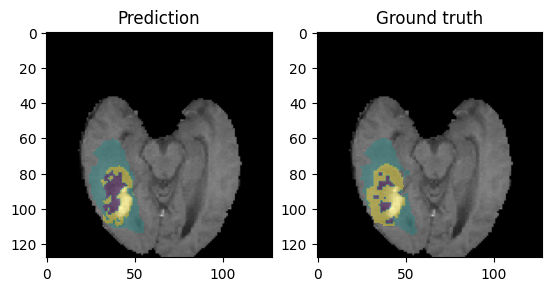
\includegraphics[width=.9\textwidth]{segmentation.png}
	\caption{Links die Segmentierung vom finalen Modell, rechts die wahrhaftige Segmentierung. (Quelle: Eigene Darstellung)}
	\label{fig:segmentation}
\end{figure}